\section{Questão 166 - Geometria, Pitágoras, Radicais}

Construir figuras de diversos tipos, apenas dobrando e cortando papel, sem cola e sem tesoura, é a arte do origami (ori = dobrar; kami = papel), que tem um significado altamente simbólico no Japão. A base do origami é o conhecimento do mundo por base do tato. Uma jovem resolveu construir um cisne usando a técnica do origami, utilizando uma folha de papel de 18 cm por 12 cm. Assim, começou por dobrar a folha conforme a figura.

\begin{figure}[H]
    \centering
    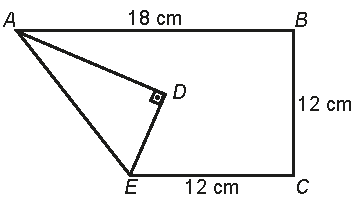
\includegraphics[width=0.15\linewidth]{Q166.pdf}
    \caption{}
    \label{fig:q166}
\end{figure}

Após essa primeira dobradura, a medida do segmento AE é

A) $ 2\sqrt{22} cm $.

B) $ 6\sqrt{3} cm $.

C) $ 12 cm $.

D) $ 6\sqrt{5} cm $.

E) $ 12\sqrt{2} cm $.

\textbf{Resolução}

\textbf{Rascunho}

\opmul[decimalsepsymbol={,},displayintermediary=all]{1.01}{1.01}\flexquad{3}
\opdiv[decimalsepsymbol={,},displayintermediary=all]{202}{1.01}\flexquad{3}
\opset{strikedecimalsepsymbol={\rlap{,}\rule[-1pt]{3pt}{0.4pt}}}
\opdiv[decimalsepsymbol={,},shiftdecimalsep=both,displayintermediary=all]{204.02}{1.0201}\quad


\begin{center}
    \href{https://youtu.be/}{
        \qrcode{https://youtu.be/}
    }\\
    Resolução: \url{https://youtu.be/}
\end{center}
